% #############################################################################
% This is Chapter 6
% !TEX root = ../main.tex
% #############################################################################
% Change the Name of the Chapter i the following line
\fancychapter{Use of synthetic speech as data augmentation}
\label{chap:6}
\cleardoublepage
Children's automatic speech recognition (ASR) poses a significant challenge due to the high variability nature of children's speech. The limited availability of training datasets hampers the effective modelling of this variability, which can be partially addressed using a text-to-speech (TTS) system for data augmentation. However, generated data may contain imperfections, potentially impacting performance. In this work, we use Adapters to handle the domain mismatch when fine-tuning with TTS data. This involves a two-step training process: training adapter layers with a frozen pre-trained model using synthetic data, then fine-tuning both adapters and the entire model with a mix of synthetic and real data, where only synthetic data passes through the adapters. Experimental results demonstrate up to 6\% relative reduction in WER compared to the straightforward use of synthetic data, indicating the effectiveness of adapter-based architectures in learning from imperfect synthetic data.

%Children automatic speech recognition (ASR) presents a significant challenge mainly due to the high variability present in children's speech, encompassing acoustic and linguistic factors. The limited availability of training datasets limits the effective modelling of these variabilities by an ASR system. In this work, we use a text-to-speech (TTS) system for data augmentation. Nevertheless, generated data are subject to imperfections from the inherent variability observed in children's speech during the training process of the TTS system. Consequently, employing the generated data directly may result in a decline in performance. Therefore, we propose to use Adapter layers to reduce the domain mismatch between real and synthetically generated data during fine-tuning. Our approach utilises adapter layers to address the domain mismatch when handling synthetic data during fine-tuning. This is achieved through a two-step training procedure. Initially, the adapter layers are trained using synthetic data while keeping the pre-trained model frozen. Subsequently, both the trained adapters and the entire model are fine-tuned using a combination of synthetic and real data, with only the synthetic data passing through the adapter layers. Results of our experiments indicate that adapter-based architectures can effectively learn from imperfect synthetic data, resulting in up to 6\% relative reduction in WER compared to the straightforward use of the synthetic data.
%Regardless of substantial advancements in automatic speech recognition (ASR), children's speech poses a significant challenge resulting in a score degradation. The primary cause for the score disparity between adult and children's speech recognition can be attributed to the considerable variability present in children's speech, encompassing acoustic and linguistic factors. Furthermore, the limited availability of training datasets limits the effective modelling of these variabilities by an ASR system. In this work, we use a text-to-speech (TTS) system for data augmentation. Nevertheless, generated data are subject to imperfections from the inherent variability observed in children's speech during the training process of the TTS system. Consequently, employing the generated data directly may result in a decline in performance. Therefore, we propose to use Adapter layers to reduce the domain mismatch between real and synthetically generated data during finetuning. Results of our experiments indicate that adapter-based architectures can effectively learn from imperfect synthetic data, resulting in up to 6\% relative reduction in WER compared to the straightforward use of the synthetic data.

\section{Introduction}
% Challenge in children speech
Advances in deep learning and large amounts of training data have greatly improved automatic speech recognition (ASR). ASR is now widely used in applications like automatic transcription and home assistants. However, the recognition of children's speech remains challenging. This is because children's speech differs significantly from adults due to developmental changes in their speech production apparatus \cite{asr-review}. These changes lead to shifts in fundamental frequencies, altered temporal and spectral characteristics, and increased disfluencies \cite{Acoustic_change_children,language_children}. Additionally, children's limited linguistic and phonetic knowledge further complicates speech recognition \cite{linguistic-children}. Finally, the scarcity of children's speech data also limits the robustness of ASR models to these variabilities.

% Improvement of children ASR
To bridge the gap between adult and children's automatic speech recognition, significant improvements have been made to the ASR pipeline. These advancements include techniques like Vocal Tract Length Normalization (VTLN) \cite{VTLN}, pitch and formant modification \cite{pitchnorm}, and adversarial multi-task learning \cite{adversarial-adapt1}. %NEW paragraph
In \cite{liao2015large}, a large dataset of children's speech, comparable in size to an adult corpus, was used to train an ASR model. This system achieved state-of-the-art performance, showcasing that neural networks can effectively learn from diverse and variable children's speech data when there is ample training data. However,
% TTS for children and Challenge in TTS for children
acquiring and annotating datasets for training speech recognition models can be notably challenging and costly, especially for children, as their attention span is limited, and they may not consistently follow prompts during reading tasks. An alternative approach is to generate synthetic datasets using a text-to-speech (TTS) model. TTS can bypass the difficulties of collecting and annotating real children's speech data. Some studies have explored TTS for ASR, either by directly using synthetic speech for training or as a form of data augmentation \cite{laptev2020you}. However, synthesizing children's speech is challenging due to their inherent substandard and imprecise pronunciation \cite{wang2021towards}. Therefore, using synthetic data directly could lead to a performance decrease \cite{wang2021towards, hu2022synt++}. %NEW added references


% Our Approach
In this paper, we introduce a novel technique called "Adapter double-way fine-tuning" to enhance ASR models for children, even when using imperfect data augmentation. Our approach involves adding additional adapter layers to the existing ASR model during fine-tuning, similar to \cite{fan2022draft}. These adapter layers are customised to address the domain mismatch between real and synthetic data. We achieve this through a two-step training procedure. In the first step, the adapter layers are trained exclusively using synthetic data while keeping the pre-trained model frozen. In the second step, we fine-tune both the trained adapters and the entire model using a combination of synthetic and real data. Crucially, our approach differentiates between synthetic and real data during fine-tuning. Synthetic data passes through the adapter layers, while real data bypasses them. This approach enables the effective use of imperfect synthetic data to enhance ASR performance for children.


\section{Related work}
\subsection{TTS data augmentation}
%TTS data augmentation
The advancement of TTS systems, achieving human-like quality, enables effective TTS-based data augmentation in ASR. This approach, as shown in studies like \cite{ laptev2020you}, involves generating synthetic speech from text using TTS models, then combining it with real speech for training, resulting in performance enhancements. Notably, this approach is not limited to well-resourced tasks and has succeeded in low-resource scenarios, as demonstrated in \cite{casanova2022asr}. Nevertheless, TTS data augmentation offers only modest improvement due to the domain mismatch between synthetic and real speech. 
% To this end, \cite{9688218} proposed to use discrete representations based on VQ-wav2vec, allowing to mitigate the mismatch with real data and reducing speaker dependency.
In order to mitigate the mismatch with real data and to reduce speaker dependency,  the use of discrete representations based on VQ-wav2vec has been proposed \cite{9688218}.


% Children data selection
Another approach to mitigate the domain mismatch between synthetic and real speech is through the use of data selection techniques, as suggested by \cite{wang2021towards}. By selectively choosing high-quality synthetic speech data. This data selection process ensures that only the most reliable and accurate synthetic speech samples are used during data augmentation. The results presented in \cite{wang2021towards} demonstrate the effectiveness of employing i-vector speaker-embedding cosine similarity as a metric for data selection, compared to metrics like error rate, acoustic posterior, and synthetic discriminator.

% Synth++
In Synth++ \cite{hu2022synt++}, an extension to the data selection technique is proposed, by incorporating separate batch normalization statistics for real and synthetic samples. While data selection handles artefacts and over/under-sampling, double batch normalization aims to further bridge the synthetic-real data gap during training. This approach uses rejection sampling based on a DNN's output. Where the DNN is trained on a 5-dimensional features vector derived from a pre-trained ASR model, including cross-entropy loss, CTC loss \cite{CTC}, word error rate (WER), lengths of tokens in prediction text, and length of tokens in target text, offering valuable insights into speech quality and characteristics.
% However, we find out that it may not be working. HERE?
\subsection{Adapters}
% Explain adapters
Adapters were first introduced for natural language processing (NLP) tasks as a simpler alternative to full model fine-tuning \cite{houlsby}. They involve adding a small number of extra parameters to each layer of the transformer model. Unlike full fine-tuning, which modifies the entire model, adapters enable targeted adjustments within specific layers while keeping pre-trained parameters intact. These adapters typically follow a bottleneck architecture with down-projection and up-projection, as seen in Figure \ref{fig:overall}-b. The bottleneck architecture's purpose is to introduce non-linear transformations, enabling Adapters to capture task-specific features and learn task-specific modifications effectively.

Since their proposal, adapters have demonstrated effectiveness in diverse NLP tasks, including language understanding and neural machine translation \cite{philip2020monolingual}. Additionally, there is a growing interest in applying adapters to automatic speech recognition. For instance, \cite{tomanek2021residual} explored adapters for atypical speech, focusing on pathological and accented speech.
% Draft
In children's ASR, Adapters are employed within the Draft framework \cite{fan2022draft}. This approach inserts and trains Adapters at each block of a pre-trained self-supervised learning (SSL) model using an SSL loss. Subsequently, the entire model, including the Adapters, undergoes fine-tuning with ASR losses. By combining SSL pre-training, Adapters, and full fine-tuning, this approach uses the advantages of SSL, the adaptability of adapters, and task-specific fine-tuning to enhance the recognition accuracy of ASR systems for children's speech.

\section{Method}
\begin{figure*}
    \centering
    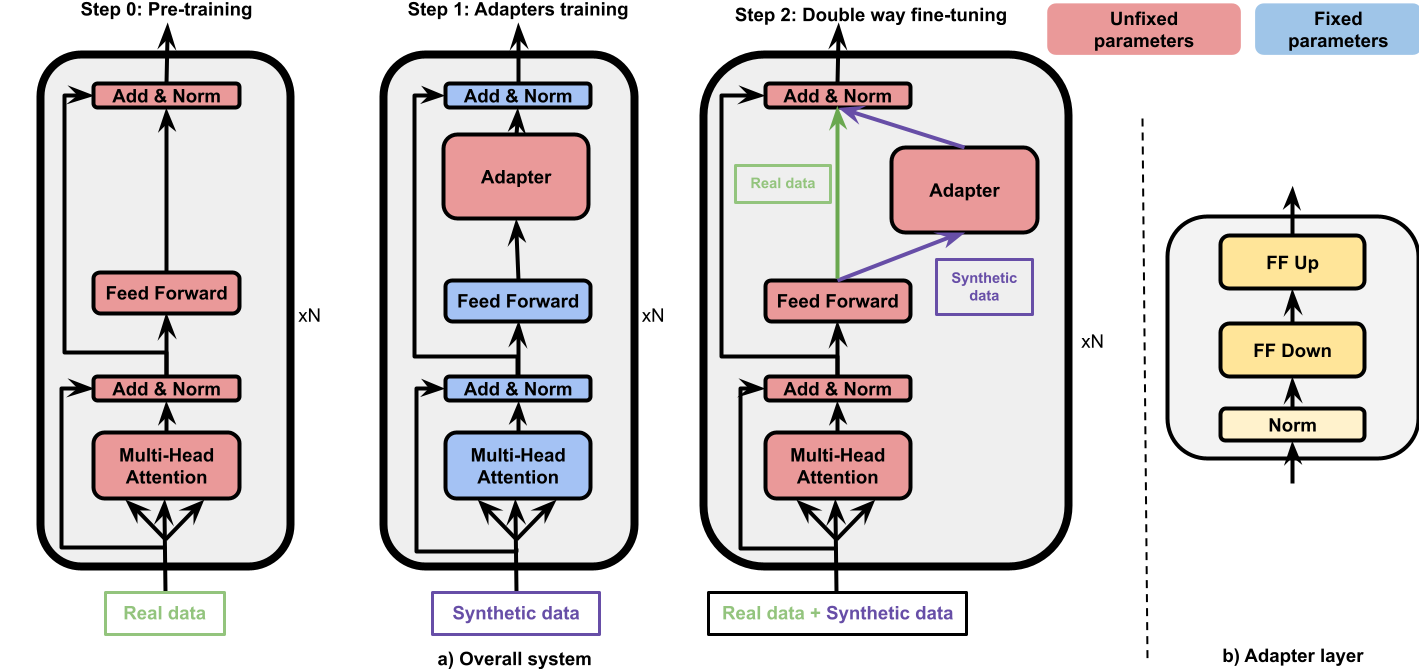
\includegraphics[width=\textwidth]{imgs/Overall_system.png}
    \caption{Overview of a) double way fine-tuning and b) Adapter layer architecture}
    \label{fig:overall}
\end{figure*}

% Motivation
Expanding on the achievements of the Draft Framework and Synth++, our approach utilizes Adapters as a substitute for the double batch normalization layer of the Synth++ framework. Our aim is to improve the performance of a pre-trained ASR model through data augmentation using synthetic data. In our methodology, we employed filtered synthetic data, implementing a speaker-embedding cosine similarity metric to retain synthetic utterances that exhibited high-quality generation. Our approach introduces two extra steps following the standard ASR model training (Step 0).%NEW
Figure \ref{fig:overall}-a provides an overview of our proposed methodology.

% Step 1
Step 1 entails training Adapter layers while keeping the ASR model parameters fixed. These Adapter layers are placed after the transformer layers' feed-forward component, aiming to learn a projection that aligns synthetic children's speech with real children's speech within the transformer layers. This step is crucial as Adapter layers require this learning process. Without it, the subsequent fine-tuning in Step 2 could be more challenging and less effective.

%Step2
In Step 2, we fine-tune both the adapters from Step 1 and the pre-trained ASR model using a mix of synthetic and real data. A crucial aspect of our approach is how we handle data flow within the model. Real samples bypass the adapter layers as they don't need further adjustments, directly passing through the original ASR model components. Synthetic data, on the other hand, goes through the adapter layers for necessary modifications to align better with real children's speech characteristics. This differential treatment of data optimises adapter usage, potentially improving the ASR system's overall performance.

% Inference
During inference, the Adapter layers become unnecessary and are discarded because the test data only contains real samples. It is important to mention that Steps 1 and 2 can be iteratively repeated with newly generated synthetic data, although this aspect is not investigated in this paper and is a subject for future research.
 
% Recap
In summary, our approach uses adapter modules to improve the performance of a pre-trained ASR model through the integration of filtered synthetic data augmentation.




\section{System description}
\label{section:SOA}
\subsection{Transformer architecture for ASR}
% Motivation children E2E
The Transformer architecture, initially developed for tasks like machine translation \cite{Transformer}, was found to be highly effective and widely used in various domains, including computer vision \cite{VIT} and language understanding \cite{Bert}. In speech recognition, it takes acoustic features as input, processes them through an encoder to create high-level representations, and uses these for token prediction in a decoder. Training typically combines a sequence-to-sequence approach with a CTC loss \cite{CTC}.
Recent studies, such as \cite{sri_end2end}, demonstrate that fine-tuning adult pre-trained Transformer-based models with children's speech data yield better results than traditional HMM-DNN based models, making the Transformer-based and End-to-end models a suitable choice for children's ASR.

In our experiments, we employed the SpeechBrain toolkit \cite{speechbrain} for the ASR part of our system, using a pre-trained Transformer model\footnote{https://huggingface.co/speechbrain/asr-transformer-transformerlm-librispeech}, trained on the LibriSpeech dataset \cite{librispeech}. This model includes 12 encoder layers and 6 decoder layers, each having a dimension of 512. Additionally, we incorporated a Transformer language model trained on a 10 million-word corpus.

\subsection{Multi-speaker text-to-speech: YourTTS}

In this work, we used the pre-trained YourTTS\footnote{https://coqui.ai/blog/tts/yourtts-zero-shot-text-synthesis-low-resource-languages} model proposed by \cite{casanova2022yourtts} based on the  Coqui toolkit. YourTTS is a TTS model that is built upon the Variational Inference with adversarial learning for end-to-end Text-to-Speech (VITS). It incorporates several novel modifications to enable zero-shot multi-speaker and multilingual synthesis. 
% Architecture
YourTTS use a 10-layer Transformer-based text encoder with 196 hidden channels. It can be used in a multilingual fashion by using a 4-dimensional language embedding concatenated with the embedding of each input character, for the purpose of our experiment, the multi-lingual aspect was discarded to only keep the English language. The decoder has four affine coupling layers, each with four WaveNet blocks for high-quality speech generation. YourTTS uses an external H/ASP speaker encoder to generate 512-dimensional speaker embeddings for individual speakers, serving as reference speakers for the model. Additionally, YourTTS incorporates a HifiGAN vocoder \cite{kong2020hifi}. As YourTTS is an end-to-end model, the vocoder is connected to the TTS model using a variational autoencoder (VAE). For a comprehensive understanding of the YourTTS architecture and training, detailed information can be found in the original paper \cite{casanova2022yourtts}.


\section{Experimental setup}
\label{section:methods}

\subsection{Real speech corpus}
\begin{table}[h!]
\caption{My Science Tutor Children Speech Corpus statistics}

\begin{center}
\begin{tabular}{r|c|c|c}
\hline
 & Training & Validation     & Test   \\ \hline
\# of utterances & 60897   & 10044    & 4079  \\ 
\# of speakers & 566   & 79    & 91  \\ 
\# of hours & 113   & 18    & 13  \\ \hline
\end{tabular}
\label{tab:statistics}
\end{center}
\end{table}
In this study, we used the My Science Tutor (MyST) Children Speech Corpus, referred to as the "Real" set. This corpus contains around 400 hours of speech collected from 1,372 students in grades three to five. It comprises conversations with a virtual tutor spanning eight scientific domains. 
%To ensure equitable domain representation, the corpus has been partitioned, with each student's data in a single partition. 
Notably, only 45\% of the utterances in the corpus are transcribed. For our experiments, we filtered out utterances shorter than one second and longer than 30 seconds due to GPU memory constraints. Additional details on the filtered corpora are provided in Table \ref{tab:statistics}.

\subsection{Synthetic data}
% Finetune YourTTS with MyST train set
To adapt YourTTS for generating children's speech, we fine-tuned YourTTS using the MyST training set. In this study, we developed two TTS systems with different parameter settings to investigate their performance and output quality under varying conditions.

The first model, referred to as TTS$_1$, underwent fine-tuning for 250 epochs without including the speaker encoder loss. In contrast, the second system, labelled TTS$_2$, was fine-tuned for 50 epochs while incorporating the speaker encoder loss. This incorporation improved the alignment between the generated speech and the reference speaker embedding provided to the model.

% Use randomly selected speaker utterances from the training set, d-vector -> TTS

The first TTS model, TTS$_1$, was used to generate 300 hours of synthetic data referred to as \textit{Synth$_1$}. The second TTS model, TTS$_2$, was employed to generate a larger volume of synthetic data, up to 1,000 hours, denoted as \textit{Synth$_2$}. To compare the performance of \textit{Synth$_1$} and \textit{Synth$_2$}, a subset of 300 hours was extracted from the \textit{Synth$_2$} dataset. The full 1,000-hour set was exclusively used to evaluate the impact of different amounts of synthetic data, both reduced and increased.

In both \textit{Synth$_1$} and \textit{Synth$_2$}, we used randomly selected d-vectors and text transcriptions from the MyST training set. Notably, the selected d-vectors did not match the associated transcriptions to introduce variability into the synthetic data.
% Use a randomly selected text transcription in order to fit the transcription style of MyST, "UM" for hesitations
We used MyST transcriptions to generate synthetic data, exposing the TTS model to its unique transcription style, including elements like "UM" hesitations. This approach helps the model learn and reproduce the specific transcription characteristics of the MyST data.
To assess the filtering effect, we generated an extra 300-hour set for both \textit{Synth$_1$} and \textit{Synth$_2$} without using speaker embedding data selection. Our data selection method relied on cosine similarity using x-vectors from a pre-trained x-vector extractor\footnote{https://huggingface.co/speechbrain/spkrec-ecapa-voxceleb}. We applied a cosine similarity threshold of 0.75 to discard bad synthetic utterances. We also explored the data selection mechanism suggested by \cite{hu2022synt++} but found it unsatisfactory, opting instead for speaker-embedding similarity as the selection criterion.

\subsection{Experiments}
We evaluated our Adapter double-way fine-tuning approach in a series of experiments, comparing it to existing methods. We started with baseline models fine-tuning an adult model to children's speech using real data for 20 and 25 epochs (step 0 in Figure \ref{fig:overall}-a).
Next, we assessed the TTS models' performances using only \textit{Synth$_1$} and \textit{Synth$_2$} data. We also explored data filtering's impact by comparing models trained on filtered and unfiltered versions of \textit{Synth$_1$} and \textit{Synth$_2$}, along with their combination with \textit{Real} data. These models were trained for 20 epochs.
We also explored double-way normalization inspired by Synt++. In one scenario, we fine-tuned the adult model for 20 epochs using a mix of filtered synthetic and real data with double-way normalization (\textit{Norm double-way from adult} in Table \ref{tab:res}). In another scenario, we trained the double-way normalization model for 5 epochs with the baseline model as initialization, referred to as \textit{Norm double-way from children}.
Finally, we implemented our \textit{Adapter double-way} approach, training the models for 5 epochs with the baseline model as initialisation. Different hyper-parameter configurations will be explored in section \ref{section:exp}.
\section{Results and discussion}
\label{section:exp}

\subsection{Comparison with existing approaches}

\begin{table}[t]
\centering
\begin{tabular}{ccc}
\hline
 Method & Synth$_1$ & Synth$_2$  \\ \hline
\multicolumn{1}{l}{\textit{Real (20 epochs)}} & \multicolumn{2}{c}{12.99\%}\\ 
\multicolumn{1}{l}{\textit{Real (25 epochs)}} & \multicolumn{2}{c}{13.15\%}\\ \hline
\multicolumn{1}{l}{\textit{Real} + Non filtered \textit{Synth}}  &   13.41\%  & 13.24\% \\ 
\multicolumn{1}{l}{\textit{Real} + \textit{Synth} \cite{wang2021towards}} & 13.09\% & 12.98\% \\
\multicolumn{1}{l}{\textit{Synth} alone}    & 40.58\%  & 40.21\%  \\ \hline
\multicolumn{1}{l}{Norm double-way (from adult)} & 12.89\% & 13.04\% \\ 
\multicolumn{1}{l}{Norm double-way (from children)} & 13.56\% & 13.87\% \\ \hline
\multicolumn{1}{l}{Adapter double-way (Ours)} &\textbf{ 12.42\%} & \textbf{12.31\%} \\ \hline
\end{tabular}

\caption{Results of the different approaches (in WER).}
\label{tab:res}
\end{table}

% Baseline
The results of the various approaches are summarized in Table \ref{tab:res}. Our baseline models achieved a WER score of 12.99\%. Training for 25 epochs led to over-fitting and a decrease in performance.
%Filtered and TTS alone
Filtered \textit{Synth$_1$} and \textit{Synth$_2$} data improved WER by 2\% compared to unfiltered data, but using only filtered TTS speech (\textit{Synth} alone) resulted in a significant 40\% WER on the \textit{Real} test set, highlighting the domain mismatch between real and synthetic.
% Double-norm 
Our experiments found that double batch normalization did not improve the baseline model's performance and even led to a 5\% relative decrease in WER  performance when evaluated with the baseline model as initialisation. This highlights the need for alternative methods to address the domain mismatch between real and synthetic speech data.
% Adapter Double-way
Our double-way adapter fine-tuning approach, initialised with the baseline model (step 0 in Figure \ref{fig:overall}), outperformed all other methods. It achieved a 4\% and 5\% relative WER improvement over the baseline on \textit{Synth$_1$} and \textit{Synth$_2$} respectively, demonstrating the effectiveness of our approach compared to longer training on the \textit{Real} set.

% TTS robustness
%In conclusion, the experiments reveal that both double-way adapters, trained using data augmentation from \textit{Synth$_1$} and \textit{Synth$_2$}, outperformed the baseline and previous works. These results demonstrate the robustness of our approach, showcasing its effectiveness across different TTS configurations.

\subsection{Effect of the number of hours}
\begin{table}[t]
\centering
\begin{tabular}{cc}
\hline
 Amount of TTS data & WER    \\ \hline
\multicolumn{1}{c}{0h} & 12.99\% \\ \hline
\multicolumn{1}{c}{10h}  &   12.73\%   \\ 
\multicolumn{1}{c}{50h}    & 12.54\%   \\ 
\multicolumn{1}{c}{100h} & 12.49\%  \\ 
\multicolumn{1}{c}{300h} & \textbf{12.31\%}  \\ 
\multicolumn{1}{c}{600h} & 12.57\%  \\ 
\multicolumn{1}{c}{1000h} & 13.14\%  \\ \hline

\end{tabular}

\caption{Results of the different number of hours in our Adapter double-way approach with \textit{Synth$_2$} data}
\label{tab:hours}
\end{table}

%Time experiments
Table \ref{tab:hours} summarizes the impact of varying amounts of synthetic data from \textit{Synth$_2$} on our adapter double-way approach. Using a small amount of synthesized speech (10 to 50 hours) yields limited ASR performance improvement. While excessive TTS data (600 to 1,000 hours) can introduce noise. Thus, it's crucial to use an appropriate amount (100 to 300 hours) to balance between robustness and avoiding noise introduction.
\subsection{Effect of the Adapters hyper-parameters}

\begin{table}[t]
\centering
\begin{tabular}{cccc}
\hline
 Location &  Bottleneck size &  5 epochs &  20 epochs     \\ \hline
\multicolumn{1}{c}{Encoder} & 64 & 12.58\% & 12.24\% \\ 
\multicolumn{1}{c}{Encoder} & 128 &  12.31\% & 12.45\%  \\ 
\multicolumn{1}{c}{Encoder} & 256  & \textbf{12.25\%} & 12.32\%  \\ 
\multicolumn{1}{c}{Encoder} & 1024 & 12.42\% & \textbf{12.22\%} \\ 
\multicolumn{1}{c}{Encoder} & 2048 & 12.57\% & 12.47\% \\ \hline
\multicolumn{1}{c}{Encoder-Decoder} & 128 & 12.45\% & 12.48\% \\ \hline
\multicolumn{1}{c}{Skip step 0} & 256 & 12.30\% & - \\ 
\multicolumn{1}{c}{Skip step 0 and 1} & 256 & 13.28\% & - \\ \hline

\end{tabular}

\caption{Results of the different configurations of Adapter double-way approach on 300h of \textit{Synth$_2$}}
\label{tab:config}
\end{table}

To assess the robustness of our approach, we assessed the Double-way adapter in diverse configurations. This involved experimenting with different bottleneck sizes (ranging from 64 to 2048), varying the number of training epochs (5 and 20), exploring the use of Adapters in the decoder of the transformer model, and conducting an ablation study by skipping step 0 and step 0 and 1.

% Best config
Table \ref{tab:config} summarizes the results, highlighting that the optimal configuration uses adapters with a size of 1024 in the encoder only, coupled with 20 training epochs, resulting in a  6\% relative WER reduction when compared to the baseline. Importantly, all configurations demonstrated superior performance to the baseline, underscoring the effectiveness of our approach.

% Other results
Our findings suggest that extended training periods were beneficial for larger Adapter bottleneck sizes, without indications of overfitting. Moreover, adding Adapters to the decoder did not significantly improve results. Finally, skipping step 0 (pre-training) did not significantly degrade results, but skipping both step 0 and step 1 (pre-training and Adapter pre-training) led to performance degradation, indicating the importance of Adapter pre-training for improved performance.

\section{Extension to Conformer architecture}


\section{Conclusions and future work}
\label{section:conclusions_tts}
We introduced the combined use of Adapters and synthetic data augmentation for children's speech recognition. Our two-step training procedure, involving training Adapter layers %with a frozen pre-trained model
using synthetic data and subsequent fine-tuning of Adapters and the entire model with a combination of synthetic and real data, yielded improvements over the baseline and previous approaches in various configurations.
%Our approach demonstrated robustness across various configurations, including TTS models, Adapter sizes, epochs, and synthetic data hours. 
or future work, we will explore an iterative approach with newly generated TTS data and varying the amount of real data used.%, and move to the Conformer architecture for ASR.

\section{Ongoing and future work} %~2-3 pages
\label{section:ongoing}
In order to answer the following research questions: \textit{Is it possible to develop an age-based, parameter-efficient automatic speech recognition model?; Is it possible to use children's synthetic speech to extend the amount of children's data? How can we control the quality and speakers’s variability?; - Given that self-supervised representation based ASR for adults matches or surpasses current state-of-the-art, are these representation appropriate for children’s speech? },
we want to pursue three research directions in the future work of this thesis: As a first direction, we want to keep exploring adapter transfer. For example, as proposed by Pfeiffer \cite{pfeiffer2020adapterfusion}, employing multiple adapters trained on different age groups or children corpus and combining them with an attention mechanism. It may also be interesting to investigate the use of explicit speaker information for robust adapter transfer \cite{gong2022layer}. Furthermore, as explained in section \ref{Vadapters}, Adapter module is structurally similar to an auto-encoder, thus it would be interesting to modify the structure of the adapter to follow the latest development in auto-encoder research. For instance, using neural discrete representations with the help of vector-quantized codebook\cite{van2017neural} at the end of the adapter's down-projection.

As a second direction we want to investigate on the use of Text-to-speech (TTS) data augmentation. Indeed, as mentioned in section \ref{section:data_scarcity}, one of the most significant obstacles in children automatic speech recognition is the lack of training data. One solution to this problem is voice conversion, in which the adult speech is transformed to child speech and then used for augmentation. However, the modified adult data can only capture a subset of the aspects of children's speech. As a result, it is important to generate children voice data directly from text \cite{wang2021towards}. A multi-speaker TTS system using speaker embeddings and  text  as input can be used to produce a synthesized utterance with the variability of child speaker. Indeed, the speaker embedding includes acoustic variability informations, which we want to find in the output utterance \cite{cooper2020zero,kim2021conditional}. One of the most challenging aspects of this approach is that the TTS model for children produces unequal quality speech due mainly to acoustic variability, and hence the ASR system suffers when trained with this additional synthetic data. Furthermore, because we intend to augment the original data with TTS data, there may be a domain shift that worsens the ASR performance. To address both of these concerns, a speaker embedding-based data selection method has been suggested, based on the computation of the cosine-similarity between the input speaker embedding and the speaker embedding obtained from the output utterance. \cite{wang2021towards}. More recently, in order to minimise domain shift, two separate normalisation layers have been employed, one for the original data and one for the TTS data. \cite{hu2022synt++}. In our research, we want to combine these two approaches to maximise the contribution of TTS data during training. In addition, we want to investigate whether the use of a GAN \cite{goodfellow2014generative}, which could create an artificial children embedding, could alleviate the problem of the limited number of speakers during training.
